%%%%%%%%%%%%%%%%%%%%%%%%%%%%%%%%%%%%%%%%%%%%%%%%%%%%%%%%%%%%%%%%%%%%%%%%%%%
%% This file is part of the book
%%
%% Algorithmic Graph Theory
%% http://code.google.com/p/graph-theory-algorithms-book/
%%
%% Copyright (C) 2009, 2010 Minh Van Nguyen <nguyenminh2@gmail.com>
%%
%% See the file COPYING for copying conditions.
%%%%%%%%%%%%%%%%%%%%%%%%%%%%%%%%%%%%%%%%%%%%%%%%%%%%%%%%%%%%%%%%%%%%%%%%%%%

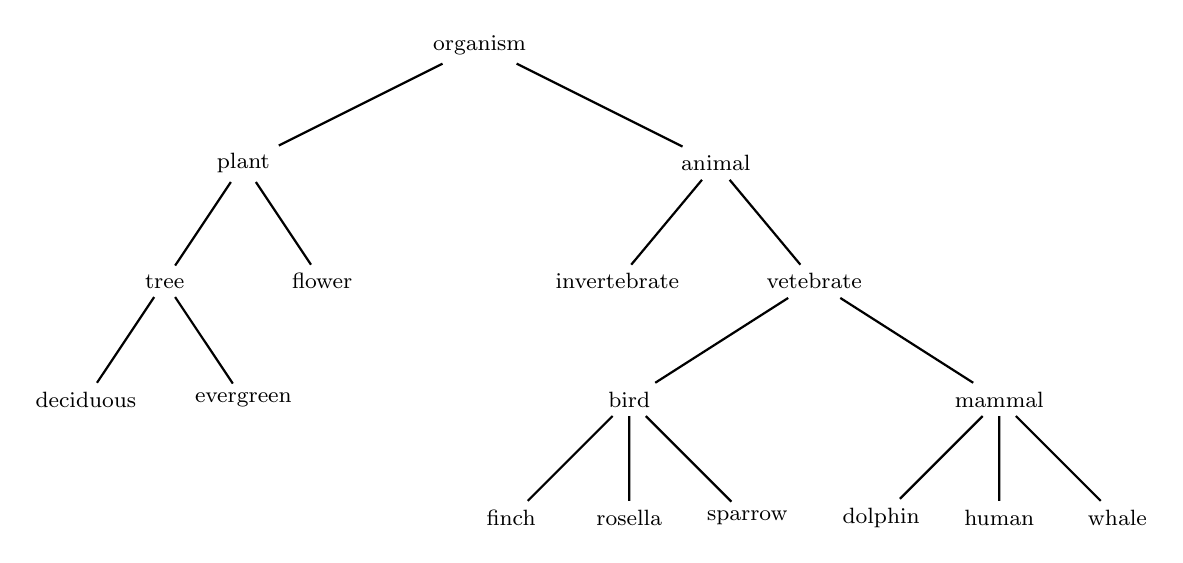
\begin{tikzpicture}
[sibling distance=6cm,-,thick]
\footnotesize
\node {organism}
  child {node {plant}
    [sibling distance=2cm]
    child {node {tree}
      child {node {deciduous}}
      child {node {evergreen}}
    }
    child {node {flower}}
  }
  child {node {animal}
    [sibling distance=2.5cm]
    child {node {invertebrate}}
    child {node {vetebrate}
      [sibling distance=4.7cm]
      child {node {bird}
        [sibling distance=1.5cm]
        child {node {finch}}
        child {node {rosella}}
        child {node {sparrow}}
      }
      child {node {mammal}
        [sibling distance=1.5cm]
        child {node {dolphin}}
        child {node {human}}
        child {node {whale}}
      }
    }
  };
\end{tikzpicture}
